\documentclass[12pt, a4paper]{ctexart}
\usepackage{graphicx, natbib}
\bibliographystyle{plain}
\usepackage{indentfirst, amsmath}
\usepackage{tikz}
%\usepackage{fancyhdr}
%\fancyhf{}
%\pagestyle{fancy}
%\fancypagestyle{fancy}{%
%	\fancyhf{}%
%	\fancyhead[C]{\fangsong 材料力学课程研究报告}
%	\fancyfoot[C]{\thepage}%
%	\renewcommand{\headrulewidth}{0pt}
%}
\usepackage{fancyhdr}
\pagestyle{fancy}
\lhead{}
\rhead{}
\chead{\fangsong 材料力学课程研究报告} 
\cfoot{}
\rfoot{\thepage} 
\renewcommand{\headrulewidth}{0.4pt} 
\renewcommand{\footrulewidth}{0pt}
\title{ 交变应力下的疲劳破坏}
\begin{document}
%%%%%%%%%%%%%%%%%%%%%%%%%%%%%%
%% 封面部分
%%%%%%%%%%%%%%%%%%%%%%%%%%%%%%
\begin{titlepage}
	\centering
	%	
\includegraphics[width=0.2\textwidth]{./templetes/image.png}\par
	%	\vspace{1cm}
	
\includegraphics[width=1.0\textwidth]{./templates/logo.png}\par
	%	\vspace{0.1cm}
	%	
\includegraphics[width=0.8\textwidth]{./templetes/title_e.png} \par
	\vspace{2cm}
	{\kaishu\LARGE 材料力学课程研究报告\par}
	\vspace{1.5cm}
	{\fontsize{36pt}{\baselineskip} \heiti 交变应力下的疲劳破坏\par}
	\vspace{4cm}
	{\fangsong\Large\itshape 吴思源\par}
	\vspace{1cm}
	{2171310846}\par
	\fangsong{自动化钱71}
	\vfill
	\vfill
	% Bottom of the page
	{\large \today\par}
\end{titlepage}
\maketitle
\section{疲劳破坏小传}

从第一次工业革命开始,疲劳就进入了理论界和工程界的研究范围。彼时由于机械设备的快速发展和机动运载工具的广泛普及,由于材料疲劳引起的事故时有发生。比如1842年5月发生的凡尔赛火车相撞事故 ( Versailles rail accident ) \citep{wiki:xxx},造成了数百人伤亡。后期调查显示,这起事故是由于前车车轴的疲劳破坏导致前车骤停,引发了多节火车车厢的追尾燃烧。

\begin{figure}[ht]	
	\centering
	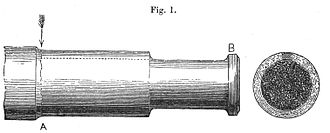
\includegraphics[scale=3.0]{31.jpg}
	\caption{轴的疲劳破坏}
	\label{fig:label}
\end{figure}

最初的观点是金属在交变应力的长期反复作用下,“累了”,引起金属塑性减小,导致脆性断裂。直到20世纪初,才借助金相显微镜观察到了微观裂纹,证明了微观裂纹是疲劳失效的根源。20世纪中叶,微观裂纹生长理论的完善和雨流计数法的发明极大程度上推进了疲劳破坏理论的发展。


\section{Comet 客机中的疲劳破坏}

由于空中的飞机受到周期性的气动载荷,使得飞机的舱体连接件也面临疲劳破坏的风险。1954年,几个月中接连数架 de Havilland Comet 客机在半空中解体坠毁,经过英国官方的调查显示,坠机原因是电子飞机导航系统天线的一个窗口发生了疲劳破坏,导致飞机外壳破裂,舱内气压骤降,造成飞机解体和舱内人员遇难。经过实验,调查人员发现窗口附近在制造中不符合要求的采用了冲孔铆接,而不是飞机最初设计中的粘合。正是由于冲孔铆接的工艺,造成了材料内部产生了裂纹源。而飞行中的反复加压降压使得材料中的裂纹不断扩展,造成了材料的脆性断裂,引发机舱失压,造成了惨剧。此外,由于机舱设计不当,在窗口附近造成了应力集中,也在这几次惨剧中起到了推波助澜的作用。\citep{wiki:xxx2}

\begin{figure}[ht]	
	\centering
	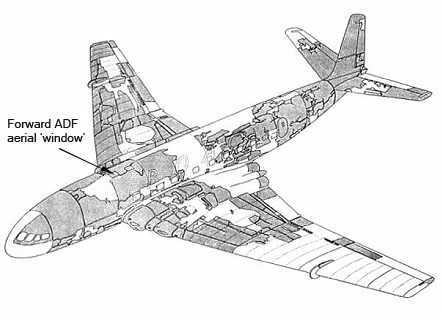
\includegraphics[scale=1.0]{32.png}
	\caption{飞机发生疲劳破坏的位置 (箭头)}
	\label{fig:label2}
\end{figure}


\section{气动载荷情况下的风力塔架}

大型海上风力机塔架通常采用圆锥筒型薄壁结构,塔架主要受到风作用下风力机风轮和塔架产生的气动载荷。除此之外,塔架也受到海浪、洋流等水动力载荷的作用。因此,塔架的疲劳载荷及疲劳寿命分析应当考虑以上多种载荷复合作用的影响。由于塔架受到外界载荷作用会发生变形与振动,这种变形与振动又反过来影响了整个风力机结构的空气动力学和结构动力学性质,使这个系统的动力学特征变得更加复杂\citep{009}。

将海上风力机塔架看成一个圆筒,作用在风轮再传递到塔架上的气动载荷是随时间变化的随机三维空间载荷,风围绕塔架的流动可以视作圆柱体绕流问题,因此根据圆柱体绕流问题的相关研究可知气动载荷是随时间和空间变化的载荷。由于海浪相对海上风力机的塔架方位角是随时间变化的,因此可以得到波浪载荷也是随时间和空间变化的载荷。根据分析,这两种载荷比较特殊,不能简单的使用疲劳强度相关理论进行分类等效计算。因此需要根据三维线性波理论进行计算,得到塔架上的随机波浪载荷;再使用处理非定常流动的相关方法,计算直接作用在塔架上的非定常气动载荷。对于疲劳寿命的估计,需要结合基本疲劳寿命曲线,采用 Palmgren Miner 的线性疲劳损伤累积法则进行计算。

\subsection{混凝土的疲劳特性}

混凝土在对称循环应力作用下的裂纹萌生寿命曲线可以近似写作幂函数形式:
\begin{equation}
S^m N = C
\end{equation}
式中,$m$ 与 $ C $ 是材料、应力幅、加载方式有关的参数。显然,取对数之后有:
\begin{equation}
\lg S = A + B \lg N
\end{equation}
这说明应力 $ S $ 和寿命 $ N $ 之间具有对数线性关系。由此可以推导出不同循环特征下的混凝土条件疲劳极限:
\begin{equation}
\left(S_{\mathrm{a}} / S_{-1}\right)+\left(S_{\mathrm{m}} / S_{\mathrm{n}}\right)=1
\end{equation}

\subsection{塔架安全寿命估算}

估算塔架的安全寿命需要结合 $ S-N $ 曲线和疲劳累积损伤准则,即 Palmgren Miner 线性疲劳寿命准则。\textbf{Palmgren Miner 线性疲劳准则: } 构件在给定应力水平反复作用下,损伤可以认为与应力循环线性累积的关系,当损伤累积到某一临界值时,就产生破坏,即: 
\begin{equation}\label{equ:1}
D(T)=\sum_{t_{1}} \frac{n\left(S_{k}\right)}{N\left(S_{k}\right)} \leq 1
\end{equation}
其中, $ S_k $ 为对称循环应力,单位为 $ \textnormal N/\textnormal m^2 $ ; $ n(S_k) $ 为实际循环数;$ N(S_k) $ 为破坏寿命;$ D(T) $ 为典型周期内的总损伤。由此结合\eqref{equ:1}可以得到\eqref{eq:2}
\begin{equation}
D(T)=\frac{1}{C} \sum_{i_{k}} n\left(S_{k}\right) S_{k}^{m} \label{eq:2}
\end{equation}

\section{钻井平台的倾覆}

\begin{figure}[ht]	
	\centering
	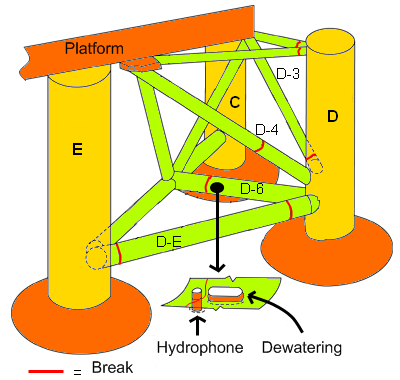
\includegraphics[scale=0.6]{33.png}
	\caption{事故钻井平台构造图}
	\label{fig:label3}
\end{figure}

在石油钻探中,钻井平台也面临着如上述海上风力机同样的挑战。由于海浪的方向变化速度很快,而且当恶劣天气情况下,海浪携带的能量极大,对应着构件所受的交变应力频率和应力幅很大,因此极端天气情况下海上钻井平台有可能因为构件疲劳而发生倾覆。1980年3月Ekofisk油田上的 Alexander L. Kielland 发生倾覆,造成了123人死亡的惨剧,其根因就是支持构件由于疲劳破坏导致钻机坍塌。


正如图\ref{fig:label3}所示,钻井平台的六条支撑之一的D-6由于疲劳发生断裂。后期调查表明,D-6的断裂可以追溯至平台组装时的一个 $ 6mm $ 角焊缝。它将固定声纳装置的构件与D-6连接起来。角焊缝的边缘较尖锐,使得此处发生了应力集中,加速了构件的破坏。经过调查,可以确信是焊缝中的冷裂纹、应力集中和海上的风浪共同导致了钻机的坍塌。值得指出的是,发生事故的 1980年3月27日晚,当地的风速达到40节,海浪高达12米。北海地区恶劣的天气状况对钻机构件的寿命是一个极大的考验。这次倾覆也成为了二战以来挪威水域最严重的灾难。
\bibliography{ref}

\end{document}
